\section{Reale Bauteile}

\subsection{Impedanzen -- Übersicht}

$$ \boxed{ Z_C = \frac{1}{\jimg \omega C} } 
    \qquad \boxed{ Z_L = \jimg \omega L } 
    \qquad \boxed{ |Z| = \sqrt{R_{\rm tot}^2 + X_{\rm tot}^2 } }
    \qquad \boxed{ f_{\rm res} = \frac{1}{2 \pi \sqrt{ R C} } } $$


\subsection{Reale Widerstände}

\begin{minipage}[c]{0.20\columnwidth}
    $$ \boxed{R = \frac{\rho \cdot l}{A}} $$
\end{minipage}
\hfill
\begin{minipage}[c]{0.78\columnwidth}
    \begin{tabular}{llc}
        $R$     & Widerstand ($@ \, 20 \, \degree$)         & $[R] = \ohm$ \\
        $\rho$  & spez. Widerstand                          & $[\rho] = \frac{\ohm \milli \meter^2}{\meter}$ \\
        $l$     & Länge des Leiters                         & $[l] = \meter$ \\
        $A$     & Querschnitt des Leiters                   & $[A] = \meter^2$
    \end{tabular}
\end{minipage}


\subsubsection{Ersatzschaltung und Frequenzabhängigkeit}

\begin{minipage}[c]{0.48\columnwidth}
    \begin{center}
\scalebox{0.7}
{
    \begin{circuitikz}[thick]
    % Ersatzschaltung für einen Reellen Widerstand
    % 
    % Author:   Alex Krieg
    % Date:     04.06.2024

    
    % Gitternetzlinien im Hintergrund
    %\draw[xstep=1cm, ystep=1cm, line width=0.1mm, color=lightgray] (0,0) grid (6,4);

    % Einstellungen für Symbole
    \ctikzset
    {  
        inductor            =   american, 
        resistor            =   european,
        inductors/scale     =   1.0, 
        capacitors/scale    =   0.8,
        diodes/scale        =   0.6,
        line width          =   0.5,
    }
    \def\labelOffset{0.4}

    % Knoten
    \coordinate (input) at (0,2);
    \coordinate (K1) at (2,2);
    \coordinate (K2) at (4,2);
    \coordinate (output) at (4.5,2);
    \coordinate (K3) at (2,1);
    \coordinate (K4) at (4,1);

    % Kreuzungspunkte
    \draw (input)   node[circ]{};
    \draw (K1)      node[circ]{};
    \draw (K2)      node[circ]{};
    \draw (output)  node[circ]{};

    % Schaltung
    %      Start Pos    Symbol type             Name    End Pos
    \draw (input)   to [L,                      l=$L_S$]  (K1);             % Spule
    \draw (K1)      to [R,                      l=$R$]  (K2);               % Widerstand
    \draw (K3)      to [capacitor,              l=$C_P$]  (K4);             % Kondensator
    \draw (K1)      to [short](K3);
    \draw (K2)      to [short](K4);

  
    \draw (K2)      to [short](output);
    \end{circuitikz}
}
\end{center}



    \begin{tabular}{ll}
        $R$     & nom. Widerstand  \\
        $L_S$   & Zuleitung \\
        $C_P$   & zwischen Anschlüssen
    \end{tabular}
\end{minipage}
\hfill
\begin{minipage}[c]{0.5\columnwidth}
    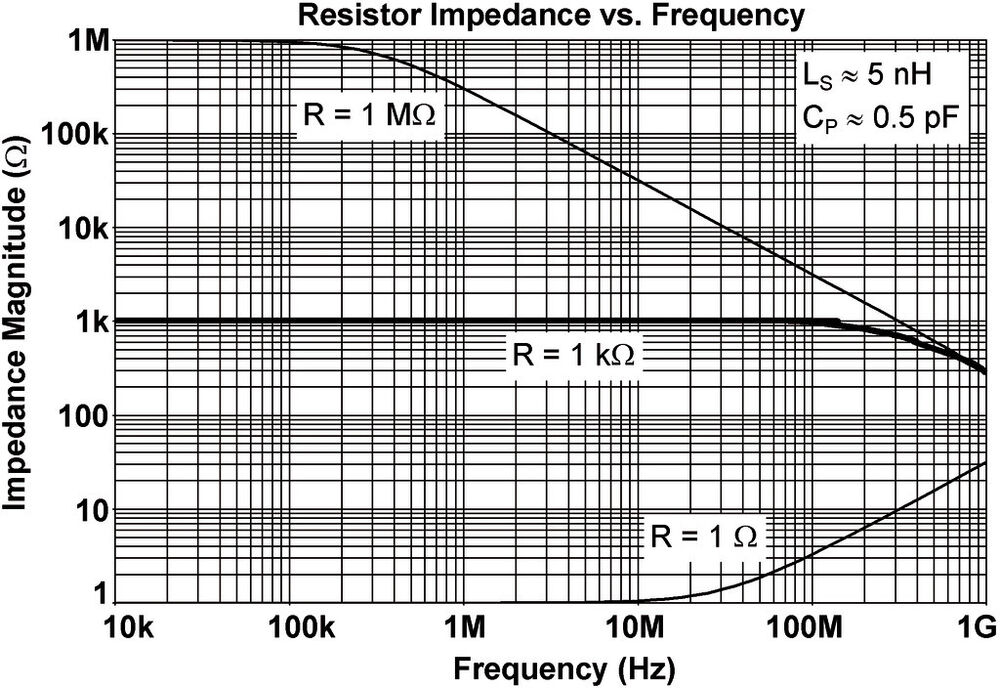
\includegraphics[width=\columnwidth]{images/realer_widerstand_frequenzverlauf.jpg}

    \begin{tabular}{ll}
        Grosse Widerstände  & \textrightarrow\ R und C \\
        Kleine Widerstände  & \textrightarrow\ R und L \\
    \end{tabular}
\end{minipage}


\subsubsection{Temperaturabhängigkeit}

%copy-paste vom Anhang
\begin{minipage}[c]{0.3\columnwidth}
    $$ \boxed{R_{\vartheta} = R_{20} + \Delta R} $$
    $$ \boxed{\Delta R = R_{20} \cdot \alpha \cdot \Delta \vartheta} $$
\end{minipage}
\hfill
\begin{minipage}[c]{0.68\columnwidth}
    \begin{tabular}{c l c}
        $R_{\vartheta}$     & Widerstand bei Temperatur $\vartheta$             & $[R_{\vartheta}] = \ohm$ \\
        $R_{20}$            & Widerstand bei $20 \, \celsius$                   & $[R_{20}] = \ohm$ \\
        $\alpha$            & Temperaturkoeffizient                             & $[\alpha] = \frac{1}{\kelvin}$\\
        $\Delta \vartheta$  & Temperaturdifferenz $\vartheta - 20 \, \celsius$  & $[\Delta \vartheta] = \celsius$\\
    \end{tabular}
\end{minipage}

\vspace{0.2cm}
\textbf{Achtung:} Leistungs-Derating bei steigender Temperatur beachten!


\begin{minipage}[t]{0.48\columnwidth}
    \subsubsection{Kenngrössen}

    \begin{itemize}
        \item Widestandswert
        \item Toleranz
        \item Temperaturkoeffizient $\alpha$
        \item max. Verlustleistung
    \end{itemize}
\end{minipage}
\hfill
\begin{minipage}[t]{0.48\columnwidth}
    \subsubsection{Auswahlkriterien}
    
    \begin{itemize}
        \item Bauform (Grösse)
        \item Leistung (Verlustwärme)
        \item Widerstandsmaterial
        \item Genauigkeit und Langlebigkeit
    \end{itemize}
\end{minipage}


\subsection{Spezielle Widerstände}


\subsubsection{Thermistoren}

Thermistoren sind \textbf{temperaturabhängige} Widerstände.

\begin{minipage}[c]{0.48\columnwidth}
    \myul{\textbf{NTC (neg. temp. Koeffizient, Heissleiter)}}

    \begin{outline}
        \1 Widerstandswert \textbf{sinkt} mit steigender Temperatur
            \2 Temperatursensoren
            \2 Einschaltstrombegrenzung
    \end{outline}

    $$ \boxed{ R = R_{20} \cdot e^{B \cdot \Big( \frac{1}{T} - \frac{1}{T_{20}} \Big)} } $$
\end{minipage}
\hfill
\begin{minipage}[c]{0.48\columnwidth}
    \myul{\textbf{PTC (pos. temp. Koeffizient, Kaltleiter)}}

    \begin{outline}
        \1 Widerstandswert \textbf{steigt} mit steigender Temperatur
            \2 Temperatursensoren
            \2 Selbst-rückstellende Sicherungen
            \2 Selbst-regelndes Heizelement
    \end{outline}

    $$ \boxed{ R = R_{20} \cdot ( 1 + A \cdot \vartheta + b \cdot \vartheta^2) } $$
\end{minipage}


\subsubsection{Varistoren}

Varistoren sind \textbf{spannungsabhängige} Widerstände.

\begin{outline}
    \1 Alternativ: Voltage Dependent Resistor (VDR)
    \1 Verringern Widerstand bei steigender Spannung (Verhalten sich wie Z-Diode aber für beide Polaritäten)
    \1 Eingesetzt für:
        \2 Begrenzung von Überspannungs-Impulsen
        \2 Eingangs-Schutzschaltungen
\end{outline}    


\subsubsection{Fotowiderstände (LDR)}

\begin{outline}
    \1 Light Dependent Resistor (LDR)
    \1 Trifft Licht auf die foto-empfindliche Fläche des Fotowiderstands, so verringert sich der Widerstand durch den 
        inneren foto-elektrischen Effekt
    \1 Relativ langsame Widerstands-Änderung
        \2 Mehrere $\milli \second$ Verzögerung
    \1 Heutzutags werden statt LDRs meist Photodioden eingesetzt
\end{outline}


\subsubsection{Druck- und dehnungsabhängige Widerstände}

\begin{itemize}
    \item \textbf{Dehnmessstreifen} (Strain Gage, Strain Gauge)
    \item Ändern ihren Widerstandswert in Abhängigkeit ihrer Dehnung bzw. Zugspannung
    \item Folienwiderstände, welche aufgeklebt werden
    \item Häufig in Brückenschaltungen verwendet 
\end{itemize}


\subsubsection{Verstellbare Widerstände, Potentiometer}

\begin{outline}
    \1 Fester Widerstand mit Abgriff dazwischen (\textrightarrow\ 'Spannungsteiler')
    \1 Potentiometer geeignet für häufiges Verstellen
        \2 Alternative heute: Digitale Potentiometer
    \1 Trimmpotentiometer nur für gelegentliches Verstellen geeignet
        \2 Alternative heute: Winkelencoder mit Hall-Sensor
\end{outline}


\subsection{Reale Kondensatoren}

\begin{minipage}[c]{0.20\columnwidth}
    $$ \boxed{C = \frac{\varepsilon_0 \cdot \varepsilon_r \cdot A}{d}} $$
\end{minipage}
\hfill
\begin{minipage}[c]{0.78\columnwidth}
    \begin{tabular}{llc}
        $C$             & Kapazität (\textbf{Plattenkondensator!})          & $[C] = \farad$ \\
        $\varepsilon_0$ & elektrische Feldkonstante $8.85 \cdot 10^{-12}$   & $[\varepsilon_0] = \frac{\farad}{\meter}$ \\
        $\varepsilon_r$ & relative Permittivität                            & $[\varepsilon_r] = 1$ \\
        $A$             & Fläche der Platten                                & $[A] = \meter$ \\
        $d$             & Abstand zwischen Platten                          & $[d] = \meter$
    \end{tabular}
\end{minipage}


\subsubsection{Ersatzschaltung und Frequenzabhängigkeit}

\begin{minipage}[c]{0.48\columnwidth}
    \begin{center}
\scalebox{0.7}
{
    \begin{circuitikz}[thick]
    % Ersatzschaltung für einen Reellen Kondensator
    % 
    % Author:   Alex Krieg
    % Date:     04.06.2024

    
    % Gitternetzlinien im Hintergrund
    %\draw[xstep=1cm, ystep=1cm, line width=0.1mm, color=lightgray] (0,0) grid (6,4);

    % Einstellungen für Symbole
    \ctikzset
    {  
        inductor            =   american, 
        resistor            =   european,
        inductors/scale     =   1.0, 
        capacitors/scale    =   0.8,
        diodes/scale        =   0.6,
        line width          =   0.5,
    }
    \def\labelOffset{0.4}

    % Knoten
    \coordinate (input) at (0,2);
    \coordinate (K1) at (2,2);
    \coordinate (K2) at (4,2);
    \coordinate (output) at (6,2);
    \coordinate (K3) at (2,1);
    \coordinate (K4) at (4,1);
    \coordinate (K5) at (6,2);

    % Kreuzungspunkte
    \draw (input)   node[circ]{};
    \draw (K1)      node[circ]{};
    \draw (K2)      node[circ]{};
    \draw (output)  node[circ]{};

    % Schaltung
    %      Start Pos    Symbol type             Name    End Pos
    \draw (input)   to [L,                      l=ESL]  (K1);             % Suple
    \draw (K3)      to [R,                      l=$R_{\rm leak}$]  (K4);        % Widerstand (leakage)
    \draw (K1)      to [capacitor,              l=$C$]  (K2);               % Kondensator
    \draw (K2)      to [R,                      l=ESR]  (K5);           % Widerstand (serie)
    \draw (K1)      to [short](K3);
    \draw (K2)      to [short](K4);

  
    \draw (K5)      to [short](output);
    \end{circuitikz}
}
\end{center}



    \begin{tabular}{ll@{}}
        $C$             & nom. Kapazität  \\
        $R_{\rm leak}$  & Leckströme (vernachlässigbar!) \\
        $\rm{ESR}$      & Anschlüsse, Zuleitung \\ 
        $\rm{ESL}$      & Anschlüsse, Zuleitung 
    \end{tabular}
\end{minipage}
\hfill
\begin{minipage}[c]{0.5\columnwidth}
    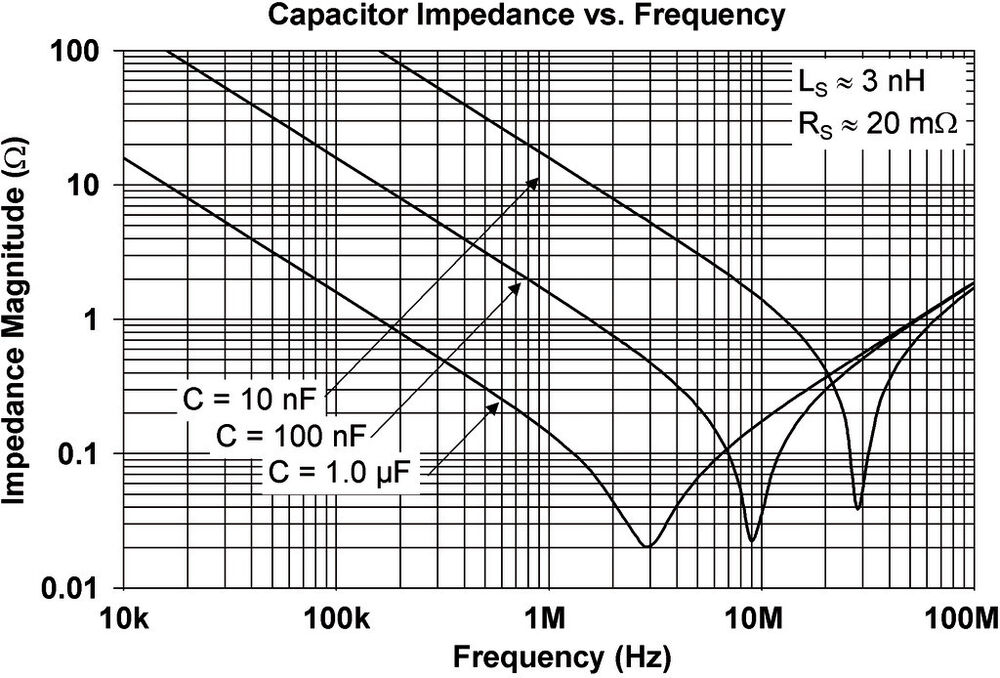
\includegraphics[width=\columnwidth]{images/realer_kondensator_frequenzverlauf.jpg}
\end{minipage}

\begin{minipage}[c]{0.48\columnwidth}
    $$ \boxed{ |Z| = \sqrt{|R|^2 + (|X_{C}| - |X_L|)^2 } } $$
\end{minipage}
\hfill
\begin{minipage}[c]{0.48\columnwidth}
    Bei Resonanz: $ |X_C| = |X_L|$ \textrightarrow\ $Z$ rein resistiv (tiefster Punkt in Diagramm)
\end{minipage}

\vspace{0.2cm}
\textbf{Hinweis: Für eine optimale Stützung der Speisung werden mehrere Kondensatoren mit verschiedenen Kapazitätswerten parallelgeschaltet}


\begin{minipage}[t]{0.48\columnwidth}
    \subsubsection{Temperaturabhängigkeit}

    \begin{itemize}
        \item Abhängig von Dielektrikum \\
            \textrightarrow\ Kennlinien
    \end{itemize}
\end{minipage}
\hfill
\begin{minipage}[t]{0.48\columnwidth}
    \subsubsection{Spannungsabhängigkeit}

    \begin{itemize}
        \item Abhängig von Dielektrikum \\
            \textrightarrow\ Kennlinien
        \item Faustregel: Je höher die maximale Spannung des kondensators, desto weniger ändert 
            die Kapazität
    \end{itemize}
\end{minipage}


\subsubsection{Verschiedene Typen von Kondensatoren}

\begin{minipage}[t]{0.48\columnwidth}
    \begin{outline}
        \1 \textbf{Elektrolytkondensatoren (Elkos)}
            \2 Gepolte Kondensatoren
            \2 Wenn bei tieferer Temperatur eingesetzt als spezifiziert: \\
                $-10 \, \celsius$ verdoppelt Lebenserwartung
        \1 \textbf{Tantalkondensatoren}
            \2 Gepolte Kondensatoren
            \2 Grosse Kapazität bei kleiner Abmessung
            \2 Tantal ist problematisch im Abbau
    \end{outline}
\end{minipage}
\hfill
\begin{minipage}[t]{0.48\columnwidth}
    \begin{outline}
        \1 \textbf{Folien-Filmkondensatoren}
            \2 Sind selbstheilend 
            \2 Hohe Genauigkeit
            \2 Relativ teuer
        \1 \textbf{Kondis mit einstellbarer Kapazität}
            \2 Zum Einstellen von Schwingfrequenzen
            \2 Trimmer
        \1 \textbf{Super-Caps}
            \2 Kapazitäten bis $3000 \, \farad$
            \2 $10 \, \%$ Energiedichte von Akkus \\
                \textrightarrow\ 10-fache Leistungsdichte 
            \2 Schnell geladen / entladen
            \2 Sehr kleine Spannungsfestigkeit
    \end{outline}
\end{minipage}


\subsection{Reale Spulen}


\subsubsection{Ersatzschaltung und Frequenzabhängigkeit}

\begin{minipage}[c]{0.58\columnwidth}
    \begin{center}
\scalebox{0.7}
{
    \begin{circuitikz}[thick]
    % Ersatzschaltung für einee Reelle Spule 
    % 
    % Author:   Alex Krieg
    % Date:     04.06.2024

    
    % Gitternetzlinien im Hintergrund
    %\draw[xstep=1cm, ystep=1cm, line width=0.1mm, color=lightgray] (0,0) grid (6,4);

    % Einstellungen für Symbole
    \ctikzset
    {  
        inductor            =   american, 
        resistor            =   european,
        inductors/scale     =   1.0, 
        capacitors/scale    =   0.8,
        diodes/scale        =   0.6,
        line width          =   0.5,
    }
    \def\labelOffset{0.4}

    % Knoten
    \coordinate (input) at (1.5,2);
    \coordinate (K1) at (2,2);
    \coordinate (K2) at (4,2);
    \coordinate (K3) at (6,2);
    \coordinate (output) at (6.5,2);
    \coordinate (K4) at (2,1);
    \coordinate (K5) at (6,1);

    % Kreuzungspunkte
    \draw (input)   node[circ]{};
    \draw (K1)      node[circ]{};

    \draw (K3)      node[circ]{};
    \draw (output)  node[circ]{};

    % Schaltung
    %      Start Pos    Symbol type             Name    End Pos
    \draw (K1)      to [L,                      l=$L$]  (K2);             % Spule
    \draw (K2)      to [R,                      l=$R_S$]  (K3);           % Widerstand
    \draw (K4)      to [capacitor,              l=$C_P$]  (K5);           % Kondensator

    \draw (input)   to [short](K1);
    \draw (K1)      to [short](K4);
    \draw (K5)      to [short](K3);
    \draw (K3)      to [short](output);
    \end{circuitikz}
}
\end{center}



    \begin{tabular}{ll}
        $R$     & nom. Widerstand  \\
        $L_S$   & Zuleitung \\
        $C$     & zwischen Anschlüssen \\
    \end{tabular}
\end{minipage}
\hfill
\begin{minipage}[c]{0.4\columnwidth}
    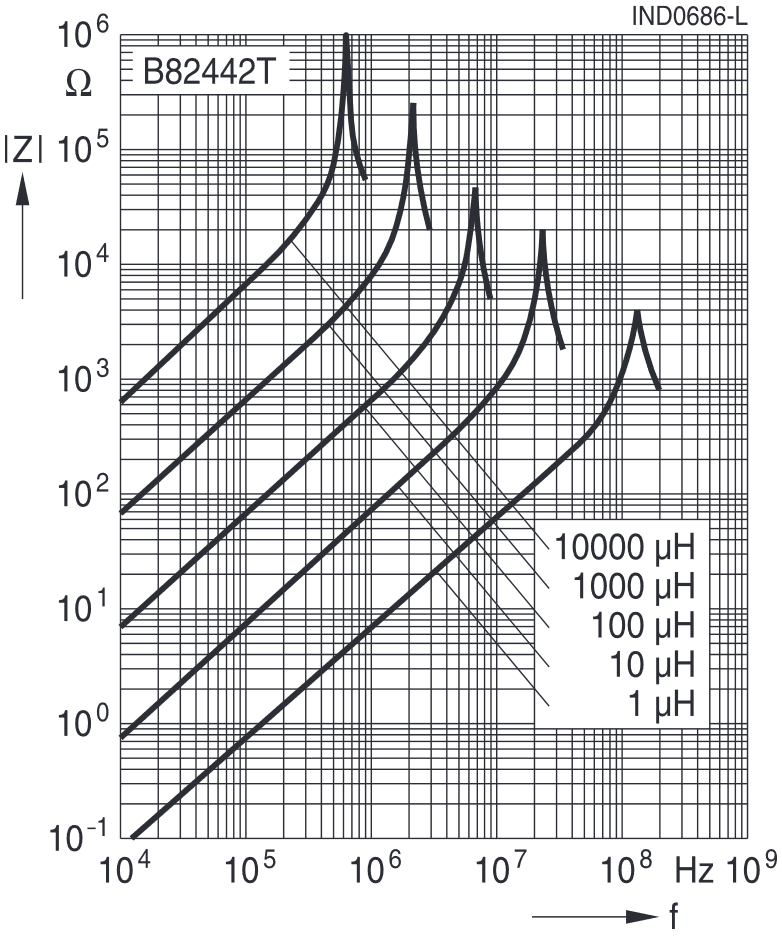
\includegraphics[width=\columnwidth]{images/reale_spule_frequenzverlauf.png}
\end{minipage}


\subsubsection{Induktivität und Strom}

\begin{minipage}[c]{0.48\columnwidth}
    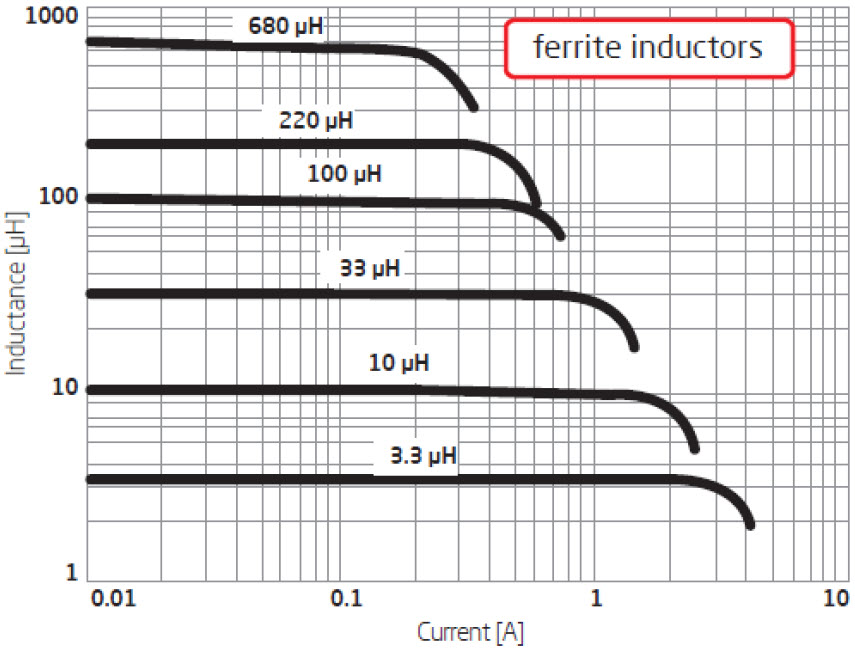
\includegraphics[width=\columnwidth]{images/induktivitaet_strom.jpg}
\end{minipage}
\hfill
\begin{minipage}[c]{0.48\columnwidth}
    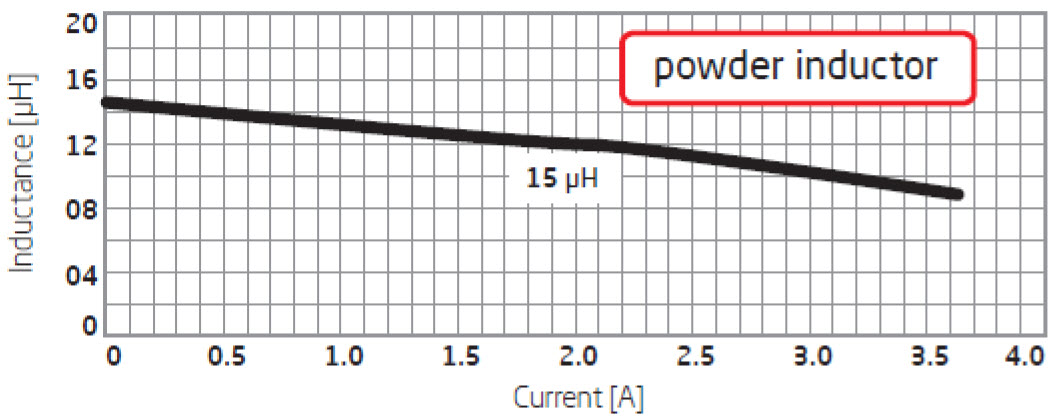
\includegraphics[width=\columnwidth]{images/induktivitaet_strom_power_inductor.jpg}

    \begin{itemize}
        \item Spule mit Ferritkern (links): \\
            Abrupter Abfall der Induktivität
        \item Spule mit Eisenkern (rechts): \\
            Kein abrupter Abfall der Induktivität
    \end{itemize}
\end{minipage}

\vspace{0.2cm}
\begin{minipage}[t]{0.48\columnwidth}
    \subsubsection{Einsatzgebiete von Spulen}

    \begin{itemize}
        \item Transformator
        \item Galvanische Trennung
        \item DC-DC-Wandler
        \item HF-Anwendungen
        \item Entstörung (EMV)
    \end{itemize}
\end{minipage}
\hfill
\begin{minipage}[t]{0.48\columnwidth}
    \subsubsection{Ferritperlen}

    \begin{outline}
        \1 Auch Ferrite Bead genannt
        \1 Dämpfung von HF-Störungen
            \2 Hohe Impedanzen bei hohen Frequenzen
            \2 Kleiner DC-Widerstand 
    \end{outline}
\end{minipage}
